\chapter{Программный комплекс оценки запаса реактивности реактора ВВР-ц}

\section{Постановка задачи}

В г. Обнинске Калужской области на базе филиала АО <<НИФХИ им. Л.Я.Карпова>> с 1964 г. находится в эксплуатации экспериментальная ядерная установка ВВР-ц -- гетерогенный водо-водяной исследовательский реактор, специализированный для проведения широкого круга исследовательских работ в области радиационной химии, структурных и материаловедческих исследований, активационного анализа, нейтронного легирования полупроводников и т.д. \cite{wwrc-2008}. 
С 1980 г. на базе реактора действует производство радионуклидов медицинского назначения, а также радиофармпрепаратов на их основе. В связи с успешностью развития данного направления и удобным географическим положением в 1986 г. было принято решение о реконструкции реактора \cite{presice-model-2011}.

В связи с необходимостью улучшения параметров реактора и повышения эффективности наработки радионуклидов (\textsuperscript{99}Мо, \textsuperscript{131}I и др.) в 2011 г. была проведена работа по созданию прецизионной нейтронно-физической расчетной модели активной зоны, отражателя реактора и органов СУЗ. 
При моделировании в полном объеме учитывается геометрия всех твэлов (топливо, оболочка, водяной зазор с соответствующими температурами), изменение изотопного состава топлива в зависимости от выгорания, геометрия и состав органов СУЗ, отражателей, экспериментальных каналов, конструкций.
Полученная прецизионная модель была верифицирована для расчета запаса реактивности реактора \cite{presice-model-2011}.

Прецизионная модель основана на методе Монте-Карло, что позволяет добиться большой точности моделирования физических процессов активной зоны реактора. 
Однако данный подход требует большого количества машинного времени для проведения вычислительных экспериментов, например, расчет запаса реактивности для одной конфигурации активной зоны занимает около восьми часов.

Кампания реактора ВВР-ц составляет 100 часов в неделю с последующей остановкой для расхолаживания, перегрузки топлива, мишеней и других технологических операций \cite{wwrc-2014}.
При такой довольно короткой кампании использование прецизионной модели для проведения оперативных расчетов довольно затруднительно: при полной утилизации одной вычислительной системы можно сделать не более 12 расчетов в течение одной кампании.
Таким образом, появляется задача по созданию программного комплекса для оценки запаса реактивности реактора ВВР-ц.
Данный программный комплекс должен помочь научно-исследовательскому персоналу реактора в проведении предварительных расчетов запаса реактивности.
К программному обеспечению предъявляется требование по кратному увеличению производительности расчета при сохранении достаточного уровня точности.
Основная задача программного комплекса сводится к аппроксимации запаса реактивности реактора в зависимости от выгорания топлива и положения органов СУЗ.

\section{Применение искусственных нейронных сетей для аппроксимации запаса рективности}

В общем виде искусственными нейронными сетями (ИНС) называется подход к построению вычислительных алгоритмов и устройств, основанный на подобии биологических нейронов \cite{NejronnyeSeti}.
В рамках данной работы будем рассматривать искусственные нейронные сети как семейство алгоритмов для обработки информации.

Искусственный нейрон (формальный нейрон) -- это элементарная
вычислительная ячейка искусственной нейронной сети. Каждый искусственный
нейрон получает вектор входных сигналов $\vec x = (x_0, x_1, \ldots, x_n)$, для которого вычисляется взвешенная сумма.
Затем от этой взвешенной суммы вычисляется значение функции активации:
\begin{equation}
    f(\sum_{i=0}^{n} \omega_i x_i + b)
\end{equation}
где $\vec\omega$ -- вектор весов, $b$ -- смещение.

Множество искусственных нейронов, получающих на вход единый вектор входных сигналов, называется полносвязным нейронным слоем.
Последовательность нейронных слоев, в которой вектор выходных сигналов предыдущего слоя является вводным вектором последующего слоя, называется многослойным персептроном.

Все веса в многослойном персептроне инициализируются случайными малыми
значениями.
В такой конфигурации персептрон производит шум в ответ на любой входной вектор. Для настройки персептрона для выполнения заданной функции производится итеративный процесс обучения.
Процесс обучения состоит в последовательном предъявлении на вход нейронной сети вектора из обучающего набора данных, получении результата на выходе нейронно сети, сравнении полученного выхода с ожидаемым выходом и корректировки весов для уменьшения полученной разницы.
Одним из наиболее часто используемых алгоритмов для обучения является градиентный спуск \cite{neuron-filatova}.

Обоснуем возможность использования искусственной нейронной сети для построения аппроксимации.
Для построения аппроксимации применима обобщенная аппроксимационная теорема. В соответствии с этой теоремой можно получить сколь угодно точное приближение любой непрерывной функции многих переменных, используя операции сложения и умножения на число, суперпозицию функций, линейные функции, а также одну произвольную непрерывную нелинейную функцию одной переменной \cite{neuron-gorban}.
Поскольку указанные операции полностью реализуются искусственной нейронной сетью с одним нелинейным формальным нейроном, то допустимо применять искусственную нейронную сеть для построения требуемой аппроксимации.

Для подтверждения возможности аппроксимации запаса реактивности с
помощью ИНС было проведено два вычислительных эксперимента.
В первом эксперименте искусственная нейронная сеть была обучена на данных, рассчитанных с помощью прецизионной модели.
Во втором эксперименте искусственна нейронная сеть была обучена на реальных данных кампаний реактора ВВР-ц.

\section{Аппроксимация модельных данных}

Для проведения эксперимента по аппроксимации модельных данных искусственной нейронной сетью был построен набор данных.
С помощью прецизионной модели были проведены вычислительные эксперименты для 34-х различных конфигураций реактора (выгорание ТВС, положения СУЗ) и для каждой конфигурации получено значение запаса реактивности.
Из полученного набора данных была сформирована обучающая выборка (25 конфигураций) и тестовая выборка (9 конфигураций).
Для конечной верификации использовались все 34 конфигурации активной зоны.

Для проведения эксперимента была создана трехслойная искусственная
нейронная сеть. Входной слой состоит из 50-ти формальных нейронов с
функцией активации ReLu:
\begin{equation}
    \label{e:relu}
    ReLu(x)=
    \begin{cases}
        0, & \text{при $x<0$;} \\
        x, & \text{при $x\ge0$.}
    \end{cases}
\end{equation}
Скрытый слой состоит из 10-ти формальных нейронов с функцией активации ReLu~(\ref{e:relu}).
Выходной слой состоит из одного формального нейрона с
логистической функцией активации:
\begin{equation}
    \label{e:logist}
    f(x)=\frac{1}{1+e^{-x}}
\end{equation}

Для обучения искусственной нейронной сети было проведено 50000 эпох обучения.
Проводилось обучение методом обратного распространения ошибки по среднеквадратичной ошибке на обучающей выборке.
Через каждые 100 эпох проводилась оценка среднеквадратичной ошибки на тестовой выборке.
В течение всего процесса обучения ошибка сходилась к нулю без расхождения.

\begin{figure}[p]
    \center{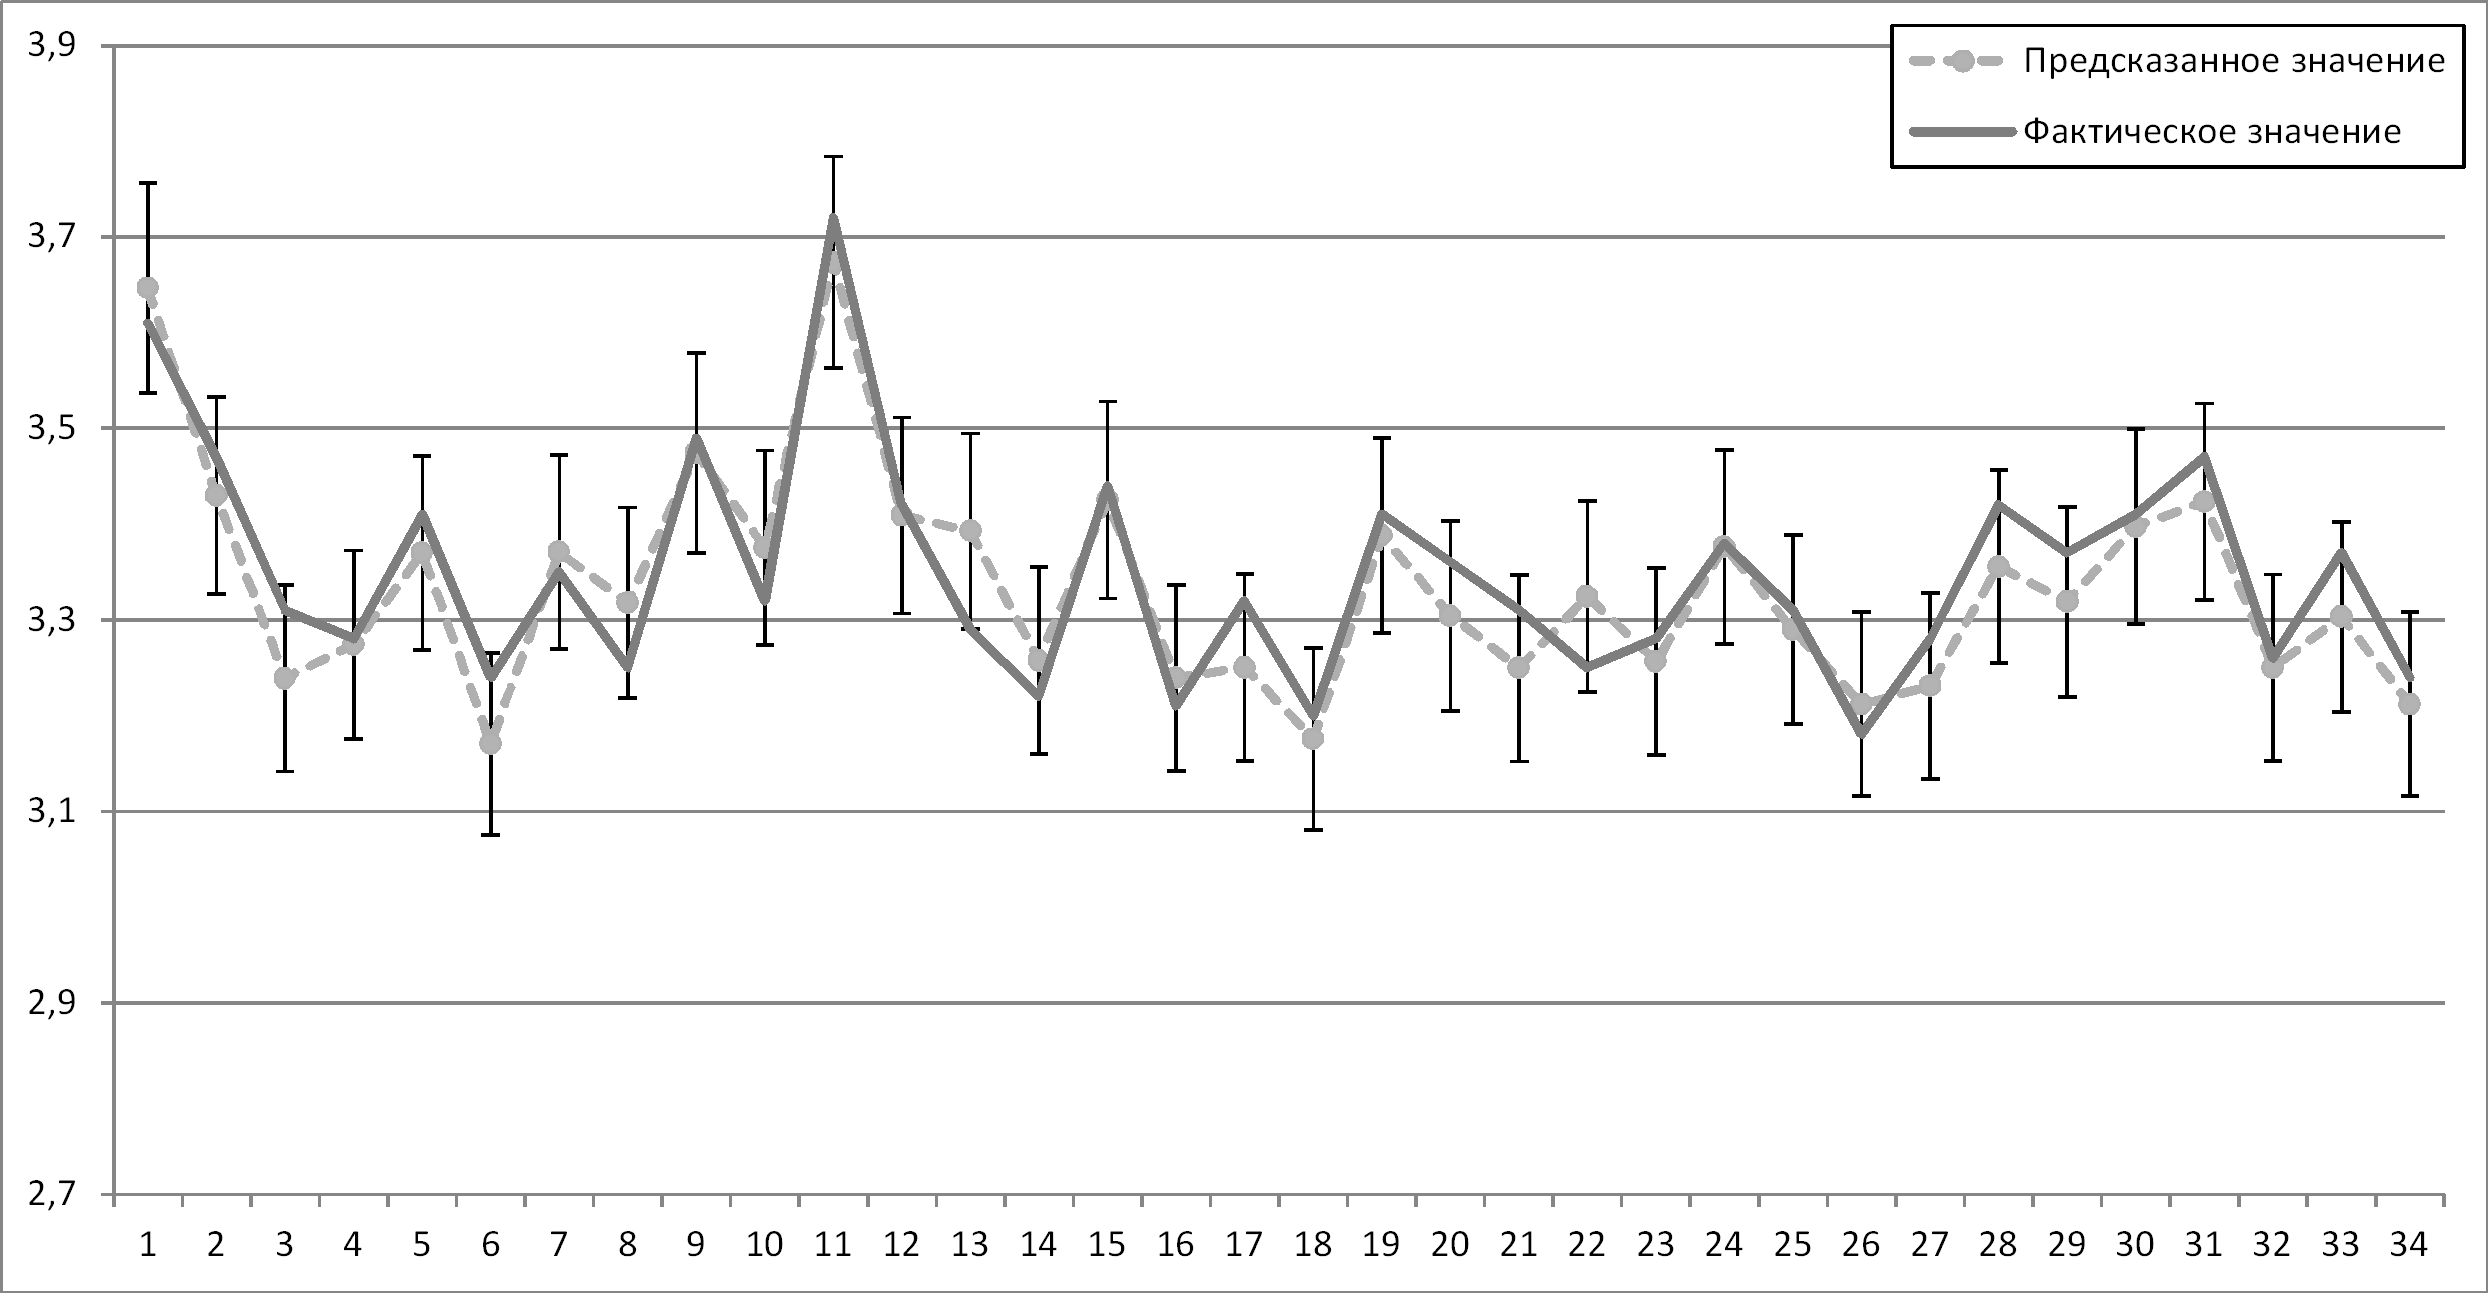
\includegraphics[width=120mm]{model-rus}}
    \caption[График верификации ИНС на модельных данных]{График верификации работы искусственной нейронной сети, обученной на модельных данных (по оси абсцисс отложены номера измерений в вариационной выборке, по оси ординат -- значение запаса реактивности,
    \% $\Delta K/K$)}
    \label{pic:model-rus}
\end{figure}

После завершения процесса обучения была проведена верификация ИНС на модельных данных.
На рис.\ref{pic:model-rus} приведены полные результаты сравнения прецизионных расчетов запаса реактивности с результатами работы ИНС.
Обобщенные результаты верификации:

\begin{itemize}
\item
  средняя абсолютная ошибка аппроксимации -- $0,0405$;
\item
  максимальная абсолютная ошибка аппроксимации -- $0,1029$;
\item
  средняя относительная ошибка аппроксимации -- $1,21\%$;
\item
  максимальная относительная ошибка аппроксимации -- $3,13\%$.
\end{itemize}

Среднее время расчета запаса реактивности с помощью искусственной
нейронной сети составляет 100 мс \cite{iop-2018}.

\section{Аппроксимация измеренных данных}

Для проведения эксперимента по аппроксимации измеренных данных для обучения были взяты данные 24-х реальных кампаний реактора.
Данные были разбиты на два набора: обучающая выборка (18 кампаний) и тестовая (6 кампаний).
Для валидации обученной ИНС использовались данные всех 24-х кампаний.

Архитектура искусственной нейронной сети идентична архитектуре в первом
эксперименте.
Для обучения ИНС было проведено 50000 эпох обучения.
Обучение также проводилось методом обратного распространения ошибки по среднеквадратичной ошибке на обучающей выборке.
Через каждые 100 эпох проводилась оценка среднеквадратичной ошибки на тестовой выборке. В течение всего процесса обучения ошибка сходилась к нулю без расхождения.

\begin{figure}[p]
    \center{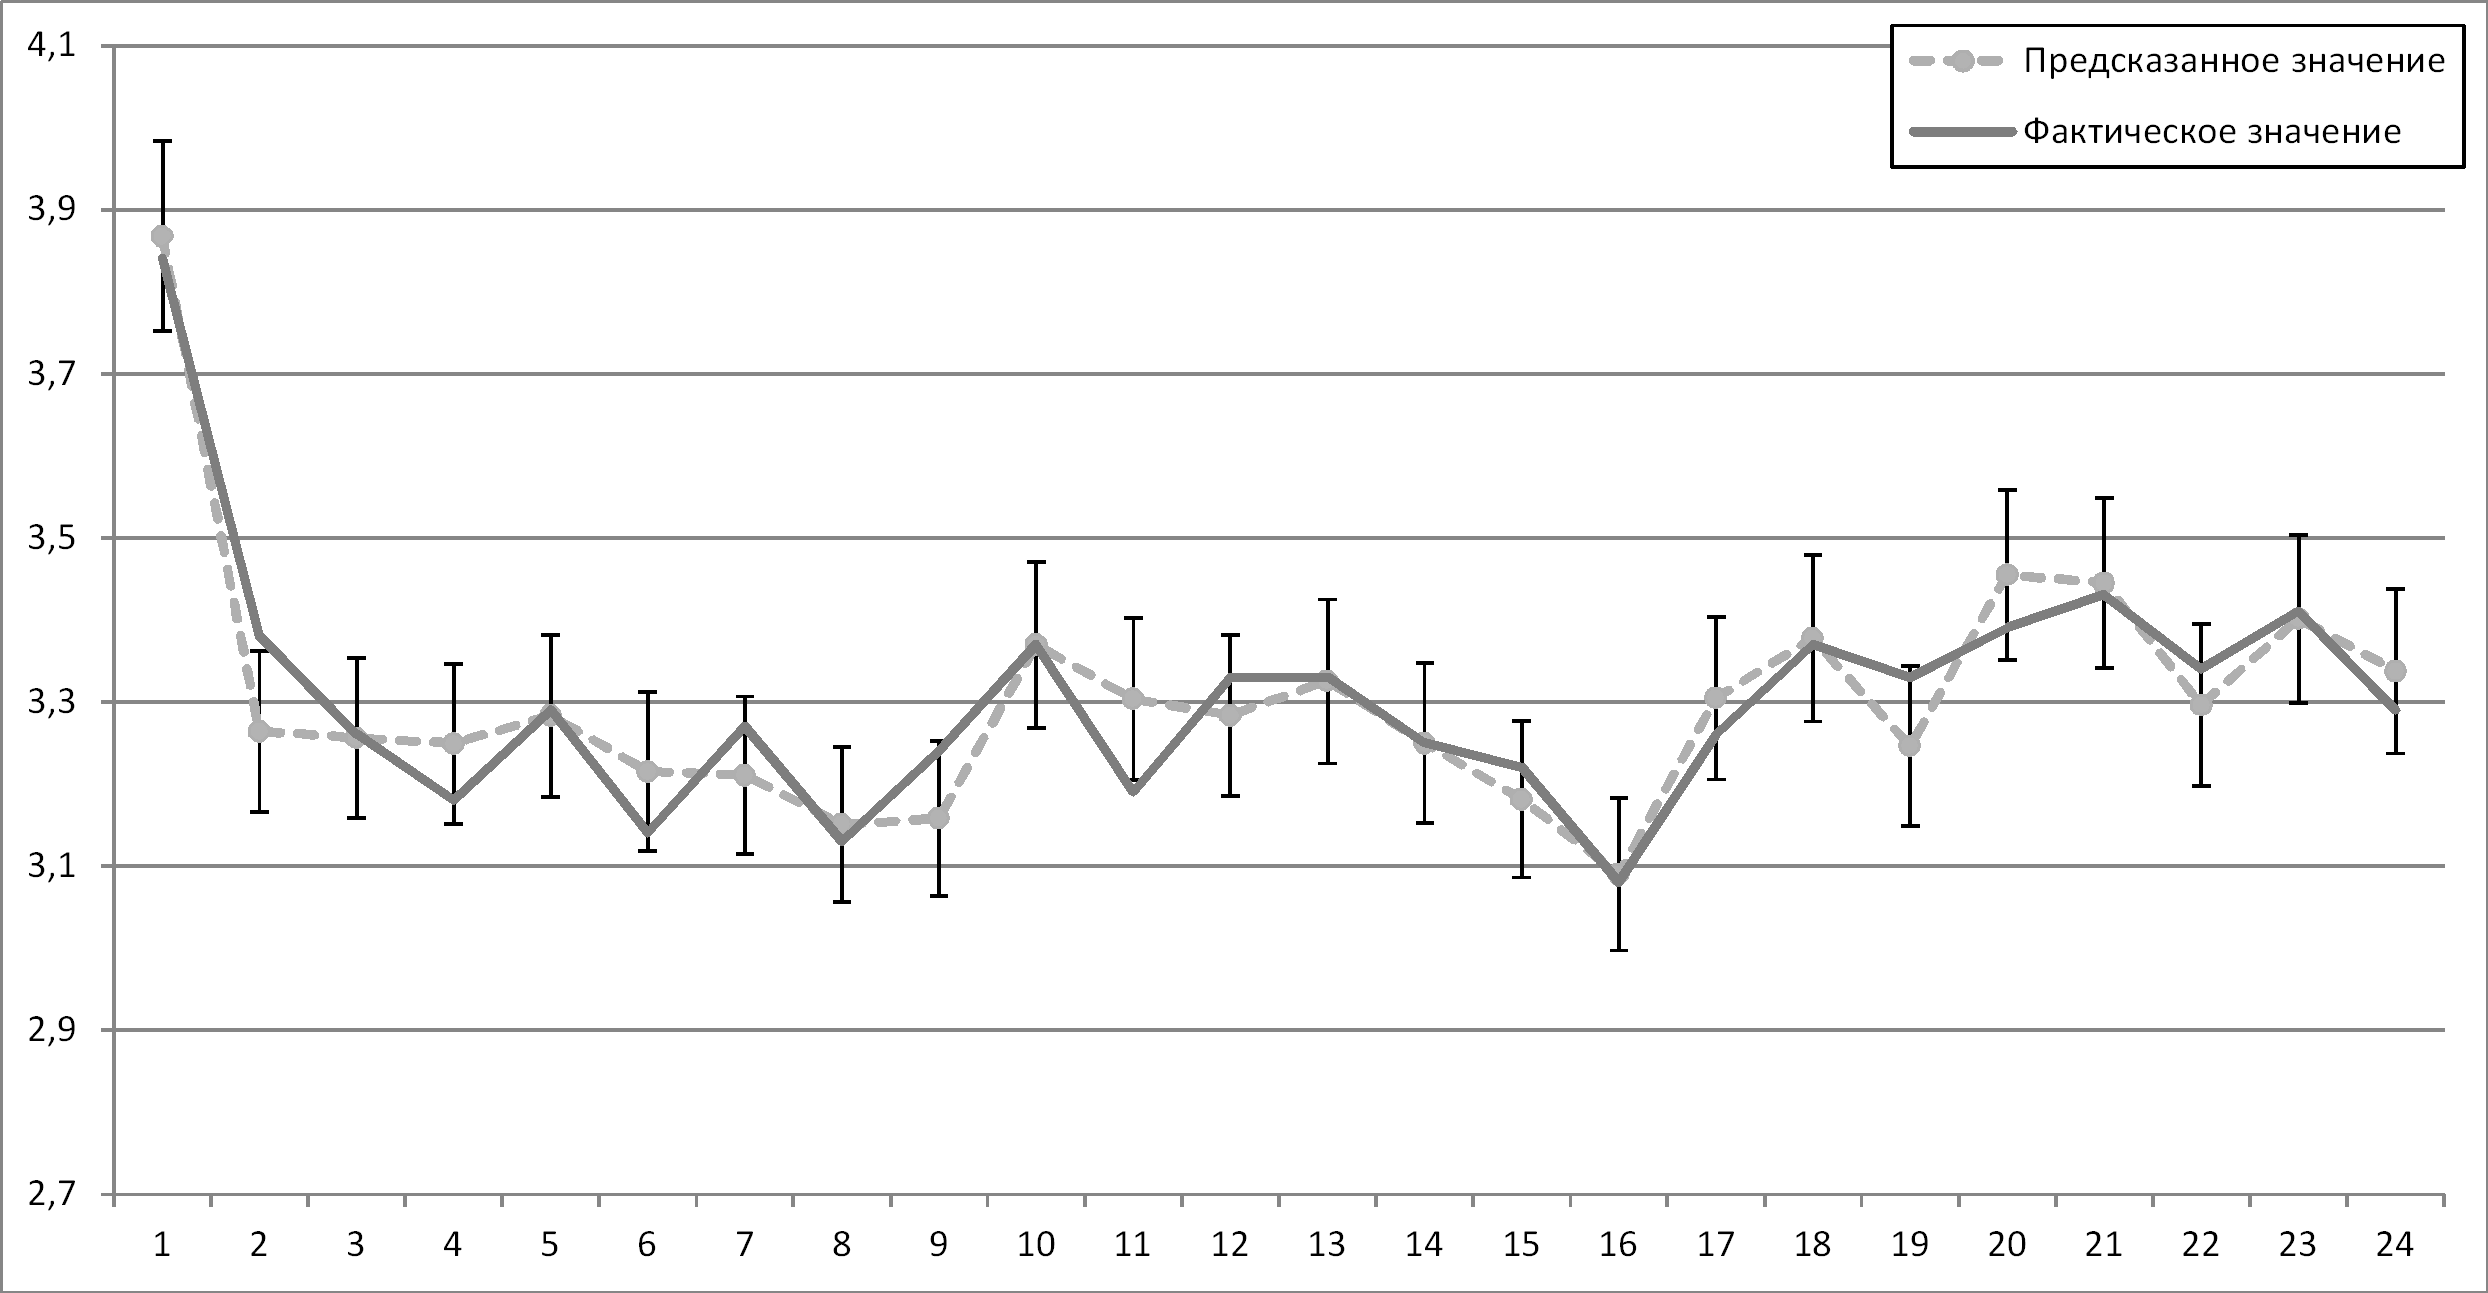
\includegraphics[width=120mm]{real-rus}}
    \caption[График валидации ИНС на измеренных данных]{График валидации работы искусственной нейронной сети, обученной
    на измеренных данных (по оси абсцисс отложены номера измерений в
    вариационной выборке, по оси ординат -- значение запаса реактивности,
    \% $\Delta K/K$)}
    \label{pic:real-rus}
\end{figure}

После завершения процесса обучения была проведена валидация ИНС на измеренных данных.
На рис.\ref{pic:real-rus} приведены полные результаты сравнения
измеренного запаса реактивности с результатами работы ИНС.
Обобщенные результаты валидации:

\begin{itemize}
\item
  средняя абсолютная ошибка аппроксимации -- $0,0412$;
\item
  максимальная абсолютная ошибка аппроксимации -- $0,1159$;
\item
  средняя относительная ошибка аппроксимации -- $1,26\%$;
\item
  максимальная относительная ошибка аппроксимации -- $3,56\%$.
\end{itemize}

Среднее время расчета запаса реактивности с помощью искусственной
нейронной сети составляет 100 мс.

В рамках описанных вычислительных экспериментов было показано, что
полученные нейросети реализуют корректную аппроксимацию, обладают
высокой точностью и скоростью работы \cite{iop-2018}.

\section{Программный комплекс оценки запаса реактивности реактора ВВР-ц}

Было показано, что на основании конечного числа прецизионных расчетов либо изменений с помощью искусственной нейронной сети можно реализовать аппроксимацию запаса реактивности реактора ВВР-ц.
Для конфигураций активной зоны реактора в рамках обучающей выборки возможно получить быструю и достаточно точную оценку запаса реактивности.

Следующим шагом необходимо обеспечить возможность использования искусственных нейронных сетей для предварительных расчетов запаса реактивности.
Для решения этой задачи разработан программный комплекс оценки запаса реактивности реактора ВВР-ц.

Программный комплекс оценки запаса реактивности обеспечивает следующие
требования:

\begin{itemize}
    \item
    пополнять обучающую выборку для искусственной нейронной сети;
    \item
    работать в режимах обучения и использования обученной нейронной сети;
    \item
    иметь удобный и интуитивно понятный пользовательский интерфейс;
    \item
    обладать легкостью установки и эксплуатации.
\end{itemize}

\begin{figure}[p]
    \center{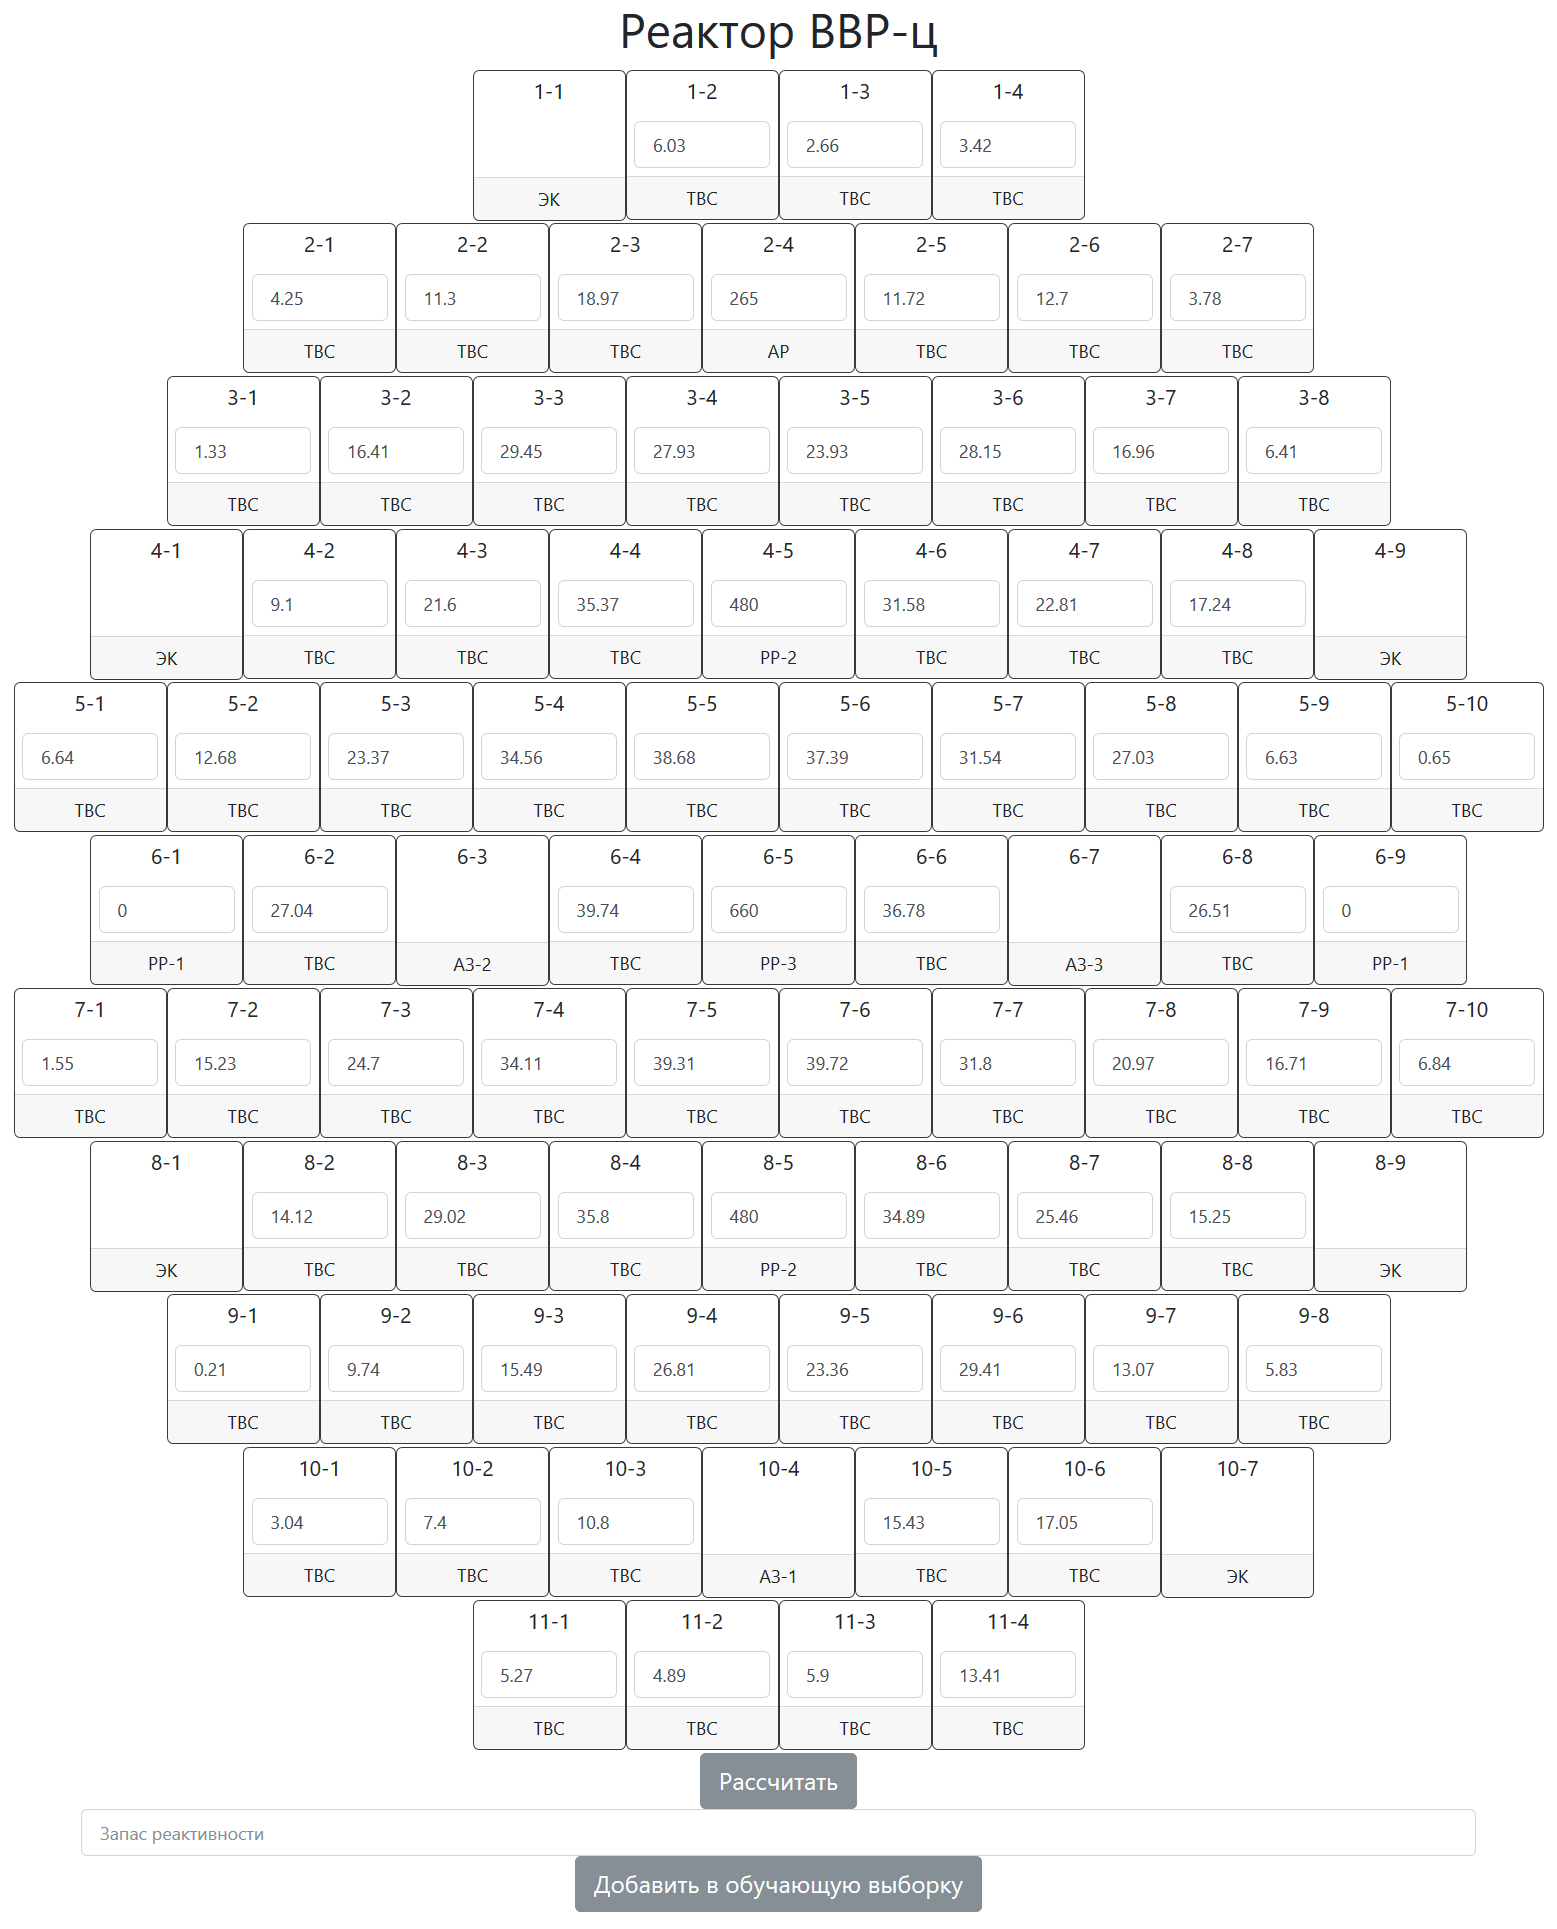
\includegraphics[width=120mm]{wwrc-gui}}
    \caption[Интерфейс программного комплекса оценки запаса реактивности]{Интерфейс программного комплекса оценки запаса реактивности}
    \label{pic:wwrc-gui}
\end{figure}

Разработанный программный комплекс состоит из следующих структурных
элементов:
\begin{itemize}
    \item искусственная нейронная сеть;
    \item хранилище данных для обучения;
    \item REST API для обмена данными;
    \item пользовательский интерфейс.
\end{itemize}

Рассмотрим эти элементы подробно.

В качестве основы для построения искусственной нейронной сети
использован фреймворк TensorFlow\cite{tensorflow2015-whitepaper,tenosrflow-2017,gs-tensorflow-2016}, который строит и исполняет граф вычислений в гетерогенных вычислительных системах, имеет богатую библиотеку примитивов для построения искусственных нейронных сетей и обеспечивает эффективное использование доступных вычислительных сред.

С помощью примитива DNNRegressor из библиотеки TensorFlow создана
искусственная нейронная сеть.
Входной слой сети -- 50 формальных нейронов с функцией активации ReLu, скрытый слой -- 10 формальных нейронов с функций активации ReLu, выходной слой -- один формальный нейрон с логистической функцией активации.
Таким образом, структура нейронной сети полностью повторяет архитектуру сети, использованную в вычислительных экспериментах.

Примитив DNNRegressor может функционировать в режимах обучения, оценки и
предсказания.

Для обучения сети DNNRegressor применяет режимы обучения и оценки, а для использования ИНС -- режим предсказания.
Предварительно обученный примитив DNNRegressor сохраняет в файле tfdata, где содержатся описание графа предсказания (Inference) и все весовые коэффициенты формальных нейронов.

Для хранения обучающих данных используются файлы формата Comma-separated
Values (CSV).
Каждая запись представляет собой строку, в которую последовательно записаны проценты выгорания каждой ТВС, положения СУЗ, а также значение запаса реактивности при данной конфигурации активной зоны.
Для проведения процедуры обучения данные из CSV-файлов загружаются в память в виде массивов NumPy.

Для обеспечения взаимодействия с пользователями программного комплекса с
помощью библиотеки VueJs реализован веб-интерфейс управления\cite{vuejs,vuejs-2017,vuejs-2016}, представляющий собой упрощенный вид картограммы реактора. В каждой из ТВС можно указать процент выгорания, а для каждого органа СУЗ -- положение (см. рис.~\ref{pic:wwrc-gui})).
В зависимости от выбранного режима работы будет либо произведена оценка запаса критичности реактора в данной конфигурации, либо добавлено еще одно значение в обучающую выборку. 
Для обеспечения связи между частями программного комплекта с помощью библиотеки Flask\cite{flask,flask-2018,flask-2016} реализован программный интерфейс
приложения передачи состояния представления (REST API) \cite{rest-2008,rest-2011}.

\section{Выводы}

В рамках данной работы рассмотрена возможность аппроксимации запаса
реактивности реактора с помощью полносвязной искусственной нейронной
сети в качестве предварительных расчетов; обучены две искусственные
нейронные сети на разных наборах данных (на модельных, полученных с
помощью прецизионной модели реактора, и на измеренных данных реальных
кампаний). Показано, что обе аппроксимации обладают достаточной
точностью для проведения предварительных расчетов запаса реактивности.
По итогам вычислительных экспериментов максимальная относительная ошибка
аппроксимации составила 3,13 и 3,56\% соответственно.

На основе обученных искусственных нейронных сетей создан программный
комплекс оценки запаса реактивности реактора ВВР-ц. Комплекс позволяет в
удобной и наглядной форме получить предсказанное нейронной сетью
значение запаса реактивности, а также пополнить обучающую выборку новыми
данными для обучения.

Программный комплекс для оценки запаса реактивности готов для
тестирования персоналом реактора ВВР-ц. Параллельно с тестированием в
данный программный комплекс можно внести ряд изменений, повышающих
удобство и безопасность эксплуатации: шифрование данных в обучающей
выборке; авторизацию, аутентификацию и аккаунтинг пользователей;
возможность ручного редактирования обучающей выборки.

Предполагается использование данного программного комплекса в виде
компонента системы автоматического планирования перезагрузки реактора. С
незначительными изменениями комплекс можно применять для реакторных
установок других типов.